\chapter{Geolocalizaci\'on} % (fold)
\label{cha:geolocalizacion}
  La Geolocalizaci\'on o Georreferenciación es un termino bastante nuevo, de hecho no aparece en el diccionario de la Real Academia Espa\~nola, no obstante se lo puede definir como:
  \begin{quote}
    El posicionamiento en el que se define la localización de un objeto espacial (representado mediante un punto, vector, área, volumen) en un sistema de coordenadas y datum determinado. Este proceso es utilizado frecuentemente en los Sistemas de Información Geográfica.
  \end{quote}

  % Para entender esta definición se necesita explicar algunos terminos     

  La Georreferenciación era usada bastante en el ambito científico, y se necesitaba de instrumental y personal bastante cualificado para su manejo, pero en la actualidad la cantidad de dispositivos con capacidad para geolocalizar un objeto sobre la tierra es bastante comun, de hecho todos los smartphones actuales (celulares con Android, Iphones) traen integrados receptores GPS (Global Posicion System),  y sumados a la exploci\'on de aplicaciones  que integran mapas con localizaci\'on (mashups), ya que se puede tener una base de datos con informaci\'on muy importante pero al final  los datos son cifras, descripciones, etc. y para tomar decisiones se hace muy difícil el interpretar estos datos, aca viene en nuestra ayuda los SIG (Sistemas de Informaci\'on Geografica).\\

  Actualmente existe una explosi\'on de aplicaciones, donde empresas, particulares y hasta donde organismos gubernamentales est\'an haciendo uso de estas tecnologías.
  Y las posibilidades son diversas, por ejemplo, se se quisiera planificar la construcci\'on de un colegio se podria integrar los datos del censo con un mapa, identificando los sectores con mayor porcentaje de ni\~nos y localizando los sectores mas propicios para realizar la construcción del inmueble. En el caso de una catástrofe natural, el tener las rutas de evacuaci\'on geolocalizadas y disponibles en un mapa de manera eficiente,  ayudaria en la evaciaci\'on de las personas del lugar.\\ 

   
  \section{Definiciones} % (fold)
  \label{sec:definiciones}
  
    En la aplicaci\'on desarrollada se requería trabajar con datos espaciales, y para ello es necesario entender algunos conceptos envueltos en el manejo de la informaci\'on geografica.

    \begin{description}
      \item[Coordenada] Es una secuencia de n-numer\'os que designa la posici\'on de un punto en un espacio n-dimensional. \\
      \item[Sistema de coordenadas] Un sistema de coordenadas es  un conjunto de reglas matemáticas que especifican como las coordenadas son asignadas  a cada  punto.
      \item[Punto] Es  la representaci\'on de una posici\'on, topol\'ogicamente 0-dimensional (no tiene volumen, area, longitud o cualquier otra unidad multi-\\dimensional).
    \end{description}

    % \subsection{Coordenada} % (fold)
    % \label{sub:coordenada}
    %   Es una secuencia de n-numer\'os que designa la posici\'on de un punto en un espacio n-dimensional. \\
    %   % one of a sequence of n-numbers designating the position of a point (4.17) in n-dimensional space
    %   % NOTA: En un 
    %   % NOTE In a coordinate reference system, the numbers shall be qualified by units.

    % % subsection coordenada (end)

    % \subsection{Sistema de coordenadas} % (fold)
    % \label{sub:sistema_de_coordenadas}
    %   Un sistema de coordenadas es  un conjunto de reglas matemáticas que especifican como las coordenadas son asignadas  a cada  punto.
    %   % set of mathematical rules for specifying how coordinates (4.3) are to be assigned to each point (4.17)

    % % subsubsection sistema_de_coordenadas (end)
    % \subsection{Punto} % (fold)
    % \label{sub:punto}
    %   Es  la representaci\'on de una posici\'on, topol\'ogicamente 0-dimensional (no tiene volumen, area, longitud o cualquier otra unidad multi-dimensional).  
    %   % topological 0-dimensional geometric primitive (4.15), representing a position
    % % subsection punto (end)

    Estas definiciones estan desarrolladas en la especificaci\'on \textbf{Simple Feature Access}, la cual es mantenida por la OGC (Open Geospatial Consortium). Esta especificaci\'on define el conjunto de tipos de datos (puntos, linia, poligono, etc) y las operaciones o metodos necesarios para manejar estos datos.
    
  % section definiciones (end)
  \section{Sistema de Coordenadas para datos Geográficos} % (fold)
  \label{sec:sistema_de_coordenadas_para_datos_geograficos}
    Se podria pensar en un sistema de coordenadas como la forma de dar sentido a un \emph{par de coordenadas}, por ejemplo cuando se ve una locaci\'on ``\verb|POINT(-66.1457475 -17.3937285)|'', como se interpretan estos n\'umeros?.
    Podria ser la latitud y longitud del campus de la UMSS, o podria ser un sistema de a\~nos luz desde alguna estrella en el Universo.
    El sistema de coordenadas es lo que diferencia estos casos.\\


    Una aplicaci\'on que maneja datos geograficos, generalmente trabaja con sistemas de coordenadas relacionadas con la superficie terrestre, conocidas como coordenadas espaciales (coordenadas globales), que permiten representar la tierra en 3-Dimensiones (3D), ya que esta es una Esfera (elipsoide oblato), o en una representacion de la superficie terrestre en 2-Dimensiones (2D), se pueden nombrar los siguientes:

    \subsection{Coordenadas geocéntricas (X,Y,Z)} % (fold)
      \label{sub:coordenadas_geocentricas}
        También conocido como Coordenadas Cartesianas 3D, Este sistema tiene como origen el centro de la Tierra, con el eje X y el eje Y en el plano del ecuador. El eje X pasa a través del meridiano de Greenwich, y el eje Z  coincide con el eje de rotación de la Tierra.

        \begin{figure}[!hbp]
          \begin{center}
            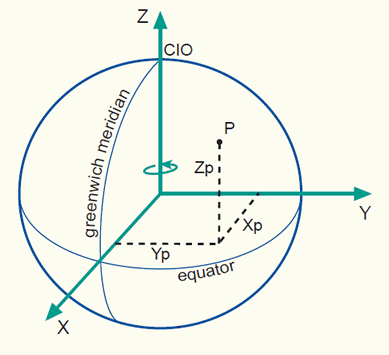
\includegraphics[width=0.7\textwidth]{coord_geocentric}
          \end{center}
          \caption[Sistema de coordenadas Geocentricas ]{Sistema de coordenadas Geocentricas, en la figura se muestra la posici\'on del punto P}
          \label{fig:coord_geocentric}
        \end{figure}

        Este Sistema de coordenadas no es muy usado en la representacion de datos.
        % , pero aveces se lo requiere para analisis de algoritmos y geometria computacional.
      % subsection coordenadas_geocentricas (end)  

      \subsection{Coordenadas Geograficas} % (fold)
      \label{sub:coordenadas_geograficas}
        Sistema de coordenadas Geográfico, utiliza las coordenadas angulares latitud  (phi o ${\phi}$) y longitud (lambda o ${\lambda}$). Este sistema de coordenadas se expresa en grados, se lo puede representar con la forma \emph{grados:minutos:segundos }\verb|(17° 23' 37.4226" S, 66° 8' 44.691" W)|, o de la forma mas comun \emph{grados decimales} \verb|(-66.1457475 S, -17.3937285 W)|.\\

        El sistema de coordenadas  mas amplimente usado, el que usan por defecto los sistemas GPS, es conocido como ``WGS 84'', y la mayoria de las aplicaciones que manejan mapas.\\

        \begin{figure}[!hbp]
          \begin{center}
            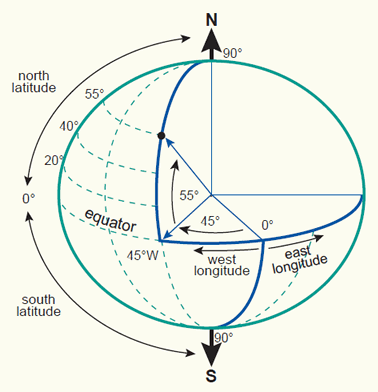
\includegraphics[width=0.7\textwidth]{coord_geographic}
          \end{center}
          \caption[Sistema de coordenadas Geográficos]{Sistema de coordenadas Geográficos, Es el sistema que maneja los mas amplimanete conocidos ``latitud y longitud''} 
          \label{fig:coord_geographic}
        \end{figure}   

      % subsection coordenadas_geograficas (end)

      \subsection{Coordenadas Proyectadas} % (fold)
      \label{sub:coordenadas_proyectadas}
        Un sistema de coordenadas proyectadas es una representación plana y bidimensional de la  tierra. Se basa en un sistema de coordenadas geográficas esf\'ericas, pero utiliza unidades de medida lineales para las coordenadas, de forma que los cálculos de distancia y área se pueden realizar en términos de esas mismas unidades.\cite{projected_ibm} \\

        Un sistema de coordenadas proyectadas requiere tomar la superficie esferica de la tierra y ``aplanarla'', este procedimiento se lo realiza con la finalidad de tener un mapa representable en una hoja de papel asi como en la pantalla de la computadora. Sin embargo este procedimiento introduce diversos tipos de distorci\'on por lo que existen diferentes clases de proyeciones que varian segun la region que se quiere representar de la Tierra.\\

        La proyecci\'on que usa Google Maps es la \textbf{Mercator Projection}, esta proyecci\'on esta dise\~nada para presevar los ángulos y las formas de las linias en forma recta, pero distorciona los tama\~nos y las distancias mientras mas lejos se encuentran de la linia del Ecuador. Esta proyecci\'on se puede apreciar en la figura \ref{fig:mercator_proyection}

        \begin{figure}[!hbp]
          \begin{center}
            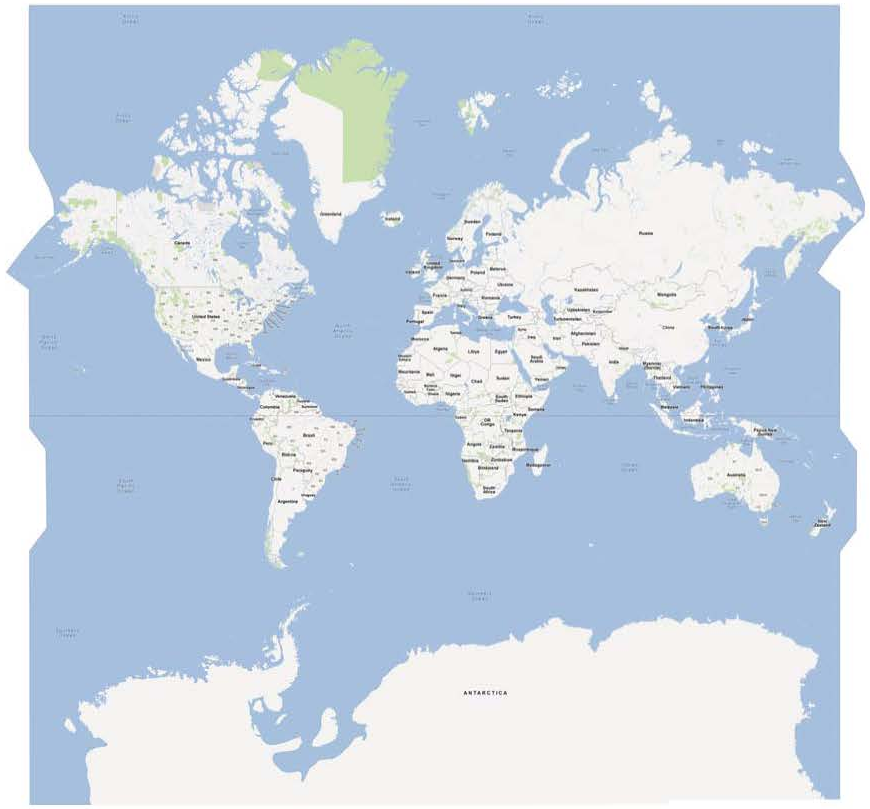
\includegraphics[width=0.6\textwidth]{mercator_proyection}
          \end{center}
          \caption[Sistema de coordenadas Proyectadas]{Google Maps usa la Proyección de Mercator para mostrar su mapa} 
          \label{fig:mercator_proyection}
        \end{figure}

        Tal como se puede apreciar en la figura \ref{fig:mercator_proyection}, la distorcion de esta proyecci\'on se hace evidente si se observa la zona de Groenlandia ya que pareceria tan grande como Africa o America del Sur, cosa que no es, ya que Groenlandia es casi 14 veces mas peque\~no que Africa. A pesar de esta distorci\'on tan marcada, la \textbf{Proyección de Mercator} es una de las mas usadas.
         % de hecho Google Maps usa esta proyecci\'on.
      % subsection coordenadas_proyectadas (end)
      \subsection{Que se us\'o en la Aplicaci\'on} % (fold)
      \label{sec:que_se_uso_en_la_aplicacion}
        Es importante entender las diferencias entre los distintos tipos de sistemas de coordenadas porque computacionalmente realizar operaciones sobre los sistemas de coordenadas tiene un costo.        
        Si se usara el sistema de coordenadas geográfico (WSG84) este es el más apropiado si se necesitaria usar grandes extensiones de la superficie terrestre, que al ser una estructura elipsoidal el costo computacional para realizar las operaciones matemáticas de calcular distancias, intersecciones, etc. es más elevado. En cambio el uso de un sistema de coordenadas proyectado (Mercator Projection) tiene un costo computacional más bajo, ya que se estaría trabajando con un sistema geométrico.\\

        % Por otro lado, 
        También hay tomar en cuenta la base de datos, ya que será esta la que se encargara de manejar los datos espaciales. Al estar usando PostGIS, se puede ver que en su documentacion\footnote{ http://postgis.org/documentation/manual-1.5/ch04.html} que claramente exorta el uso de un sistema geometrico sobre el uso de un sistema geografico si  se va trabajar con datos que cubran una peque\~na area geografica. Tomando en cuenta esta recomendaci\'on y el tama\~no del área de estudio (campus UMSS), se procedió a implementar en la base de datos el uso de la proyecci\'on Mercator. Se va usar Mercator sobre las otras proyecciones porque aparte de las ventajas que se mencionaron con anterioridad, Google Maps usa esta proyecci\'on y ya que se usara este mapa lo más correcto es trabajar con la misma proyecci\'on.  
       

        % Como 
        % PostGIS maneja dos tipos de datos, geograficos y geometricos

      % section que_se_uso_en_la_aplicacion (end)
  % section sistema_de_coordenadas_para_datos_geograficos (end)
  \section{Tipo de archivos} % (fold)
  \label{sec:tipo_de_archivos}
  
  % section tipo_de_archivos (end)

  \section{Implementaci\'on} % (fold)
  \label{sec:Implementacion}
    Al implementar una aplicaci\'on con Rails, no se maneja la base de datos con ordenes SQL  puro. La base de datos se la maneja atraves de un ORM (ActiveRecord). 
    Para llevar a cabo esta tarea es necesario escribir una \emph{migraci\'on}, el cual es un metodo que Rails interpreta y lo traduce a ordenes SQL.\\
    \begin{center}
      \begin{verbatim}
        class CreatePlaces < ActiveRecord::Migration
          def change
            create_table :places do |t|
              t.string :name
              t.point :coord, :srid => 3785 
            end
          end
        end
      \end{verbatim}
    \end{center}
    Esta \emph{migraci\'on} cre\'o la tabla \textbf{places} con los atributos \textbf{name} y \emph{coord}, el atributo \textbf{name} es del tipo string que en PostgreSQL se traducir\'ia en una columna de tipo \emph{VARCHAR(255)}, y el atributo \textbf{coord} de tipo point con un srid\footnote{ Spatial Reference System Identifier, El SRID corresponde a un sistema de referencia espacial basado en el elipsoide concreto usado para la creación de mapas de tierra plana o de tierra redonda.\cite{msdn_srid} } 3785,     el SRID  es la llave primaria de la tabla \emph{spatial\_ref\_sys} que se crea cuando se inicializa una base de datos espacial, esta tabla provee la informaci\'on necesaria para interpretar y convertir correctamente todas las coordenadas existentes, adem\'as permite definir alg\'un tipo de sistema de coordenadas si no existe en esta tabla, el SRID 3785 esta definida en la tabla \emph{spatial\_ref\_sys}  como ``Popular Visualisation CRS / Mercator'', Rails interpreta el tipo point y crea una columna de tipo \emph{geometry}, definida por PostGIS.\\

    El anterior código escrito en Rails se traduciria en SQL de la siguiente forma: 
    \begin{center}
      \begin{verbatim}
        CREATE TABLE places (
          id    INTEGER       PRIMARY KEY,
          name  VARCHAR(255)
        );
        SELECT AddGeometryColumn(
                  'places', -- nombre_tabla
                  'coord',  -- nombre_columna
                  3785,     -- srid
                  'POINT',  -- tipo
                  3         -- dimensi\'on
               );
      \end{verbatim}
    \end{center}
    Al usar un framework como Rails, se tiene como ventaja que existen herramientas creadas, comprobadas y avaladas por una gran catidad de usuarios, en este caso se preciso de herramientas que ayuden en el  manejo de informaci\'on geogr\'afica, la gema \textbf{RGeo} \footnote{ RGeo es una libreria de datos geospaciales  para el lenguaje Ruby.} es la que maneja  la correcta manipulaci\'on de estos datos.\\

    Una ves configurada/implementada la base de datos se puede obtener la locacion de cualquier lugar mediante el ORM.

\begin{center}
  \begin{verbatim}
    $ rails console
    Loading development environment (Rails 3.2.3)
    > UMSS = Place.find_by_name("UMSS")
    => #<Place id: 21, name: "UMSS", 
        coord: #<RGeo::Geos::PointImpl:0x52e4e60 
        "POINT (-7363625.14672284 -1966786.8137609)">, ... >
    > UMSS.coord_geographic.to_s
    => "POINT (-66.14857015827988 -17.394421906929086)"
  \end{verbatim}
\end{center}

    Tal como se puede apreciar, la consola de Rails permite manipular los datos cargados en la aplicación desde la línea de comandos de Linux, en la demostración se ve que la variable \textbf{UMSS}  es el resultado de la búsqueda en la base de datos mediante el modelo Place con la opción de buscar por el nombre, el atributo \textbf{coord} de la variable \textbf{UMSS} es un objeto de tipo RGeo y  el punto está proyectado, y si fuera necesario también se puede obtener el mismo punto en coordenadas geográficas.\\
    % , como en el caso de que la aplicacion consume datos por 

    Obtener la coordenada es el primer paso, seguidamente se debe mostrarlo sobre un mapa, en este caso \emph{Google Maps}. El API de Google Maps permite este paso declarando un objeto \emph{Marker}, que es la imagen que muestra Google Maps, este objeto para mostrarse en el mapa requiere que se le declare un objeto tipo \emph{LatLong}, el cual es la coordenada y se por \'ultimo se necesita declarar el mapa en el cual se va mostrar el marcador. Este objeto es altamente personalizable pero b\'asicamente este es el procedimiento para representar la coordenada en un mapa de Google Maps. Tal como se puede apreciar en la figura \ref{fig:gmaps_geo}\\
    % \begin{center}
    %   \begin{verbatim}
    %     var maker = new google.maps.Marker({
    %       position: new google.maps.LatLng( lat, lng  )
    %       map: UMSS.map
    %     });
    %   \end{verbatim}
    % \end{center}

    \begin{figure}[!htp]
    \label{fig:gmaps_geo}
  \begin{verbatim}
    var maker = new google.maps.Marker({
      position: new google.maps.LatLng(UMSS.lat, UMSS.lng)
      map: UMSS.map
      icon: new google.maps.MarkerImage('img/gota.png');
    });
  \end{verbatim}

          \begin{center}
            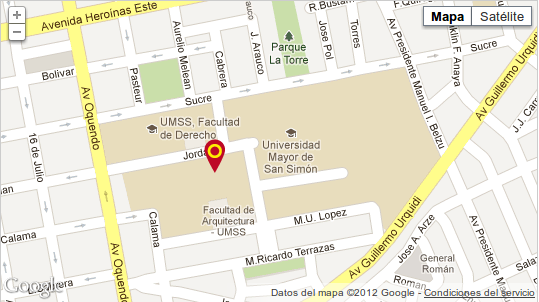
\includegraphics[width=0.9\textwidth]{gmaps_geo}
          \end{center}
          \caption[Google Maps - Marker]{Google Maps representa un \emph{punto} con un \emph{marcador}, el cual es altamente personalizable } 
    \end{figure}



    % Pero esta coordenada  no seria  facil de entender sin una adecuada representacion sobre un mapa,  


  % section Implementacion (end)
  % \section{Los datos} % (fold)
  % \label{sec:los_datos}


  %   Una vez implementada la Base de datos es necesario insertar ``los datos''
  % % section los_datos (end)


  \section{Conclusi\'on} % (fold)
  \label{sec:geo_conclusion}
    Los Mapas son herramientas muy útiles a la hora de desplegar información pero realizar el mapa, crear las fórmulas matemáticas con las cuales se trabajará, determinar cómo se usarán estas fórmulas para una representación adecuada de la superficie terrestre, es una tarea muy compleja. Como programador la tarea más complicada fue determinar el tipo de mapa y el sistema de coordenadas más adecuado al trabajo.\\

    Los términos de longitud y latitud son en un inicio, más fácilmente comprendidos que un sistema proyectado, pero no se puede tomar a la ligera una correcta comprensión del uso de los \emph{sistemas de coordenadas} en una base de datos espacial, un mal uso de estos conceptos puede generar errores a la hora de manejar datos  espaciales o en el resultado de operaciones sobre estos  datos, llegando a resultados no deseados y que pueden costar mas tiempo y dinero en una posterior correci\'on.\\

    La geolocalizaci\'on es actualmente una tecnolog\'ia y una herramienta usada en gran medida por una gran cantidad de aplicaciones web, a\~nadiendo b\'usquedas y resultados personalizados a nivel pa\'is, ciudad, barrio y calle, resultando en una gran variedad de servicios y que actualmente es de gran ayuda en diferentes escenarios. La geolocalizaci\'on nos ayuda a movernos por una ciudad, encontrar restaurantes, cines, transporte, etc. actualmente es una de las herramientas m\'as usadas y desarrolladas a nivel de industria, comercio, turismo, etc. y vale la pena estudiarla y entenderla.\\


    % Maps are deceivingly simple tools, and cartography a surprisingly complex discipline. While the most trouble many of us will have with a map is figuring out how to fold it, this simplicity belies great sophistication that has been developed over the years. 
  % section geo_conclusion (end)


  % \begin{description}
  %   % \item[SIG] Un Sistema de Informaci\'on Geografica es una manera de visualizar c\'omo es y que est\'a ocurriendo en algun lugar. La posibilidad de incorporar coordenadas con presici\'on.

  %   % A GIS is a colletion of software, normaly manipulatedby its user through a single interface, and designed to perform a wide range of operations on geographic data.  
  %   % Research  Methods in Geography
  %   % Basil Gomez and John Paul Jones III.
  %   % ISBN 978-1-4051-0710-5

  %   \item[Datum] 
  %   \item[] 
  %   \item[] 
  % \end{description}

  % procesar
  % Se tien
  % , Sistema de Posicionamiento Global por sus siglas en espa\~nol
% chapter geolocalizacion (end)

